% pathsearch.tex

\chapter{Optimal Path Determination by Exhaustive Search}
\label{chap:dijkstra}

\section{Defining an augmented $\lambda$ space}

In order to ascertain the impact of Gelman and Meng's result on alchemical intermediate selection for free energy calculations, we must first define in which way to expand the alchemical state space defined by equation \eqref{lambdascaling}. 
Numerous options exist, including separation of energy terms (Jiang \& Roux\cite{jiang2010free}) and the addition of a biasing potential (Darve et al.\cite{darve2008adaptive}), but the most natural choice is to expand the alchemical space using a temperature parameter (Sugita et al.\cite{sugita2000multidimensional}).

Using temperature as a second dimension in the alchemical state space confers numerous and predictable benefits, both practically and technically. 
Varying temperature in the alchemical space confers similar benefits to replica exchange molecular dynamics (REMD), an expanded ensemble sampling method designed to overcome energetic barriers\cite{sugita2000multidimensional}, and because temperature is a standard tunable parameter in molecular simulation packages, sampling states in this expanded space comes at no additional cost, implementation-wise.

As defined, the potential energy is not dependent on temperature, but the unnormalized density is affected:

\begin{equation} 
q_{\lambda,\beta}(\boldsymbol{x}, \lambda, \beta) = \exp(-\beta U_{\lambda}(\boldsymbol{x},\lambda))
\label{eqn: alchemical distr}
\end{equation}

\noindent Consequently, the partition function $Z_{\lambda, \beta}$ will also depend on the temperature.

While temperature is a convenient thermodynamic parameter for our purposes, letting temperature vary introduces some issues as well. Free energy differences between two states can be expressed as the log ratio of partition functions as in \eqref{freeeneqn} and \eqref{tbar} only when the two states are at the same temperature. This imposes the constraint that the end points of our alchemical path, the real physical systems of interest, must be at the same temperature.
%, but this was always the case for biologically motivated calculations.
%requirement is not problematic: it was already implicit in other methods.
What must be verified is that intermediate alchemical states can pass through regions of varying temperature while still recovering the telescoping product in \eqref{tbar}. Revisiting \eqref{tbar} when the temperature of the intermediate is given by $\beta_i$:
\begin{equation} \label{tempfail}
\Delta G=(G_2-G_i) + (G_i-G_1) = [-\beta^{-1} \log(Z_1) + \beta_i^{-1} \log(Z_i)] + [-\beta_i^{-1}\log(Z_i) +\beta^{-1}\log(Z_0)]
\end{equation}

\noindent It clear that we cannot estimate this free energy difference using BAR type methods if $\beta_i \neq \beta$.
To resolve this problem, we can define $G_i^\ast$ as scaled free energies for intermediate states:
\begin{equation} \label{Gscale}
G_i^\ast = \beta_i/\beta *G_i = \beta_i/\beta * (-\beta_i^{-1} \log(Z_i)) = -\beta^{-1} \log(Z_i)
\end{equation}

\noindent Replacing $G_i$ with $G_i^\ast$ in \eqref{tempfail} will recover the telescoping product, as in \eqref{tbar}.

It is therefore important to note that in this expanded alchemical space, we are not computing sums of ``correct" free energies along the alchemical path, but ``improper" free energies. 
Only the sum of free energies along a complete path is physically meaningful.
Nevertheless, this expanded space has been shown to be well suited to relative free energy calculations using BAR, since these improper free energies allow for the estimation of a telescoping product of normalizing constants, which are unaffected by the scaling in \eqref{Gscale}.

\section{Revisiting Gelman and Meng in discrete state spaces}

To demonstrate the existence of better paths in our augmented $(\lambda, T)$ space, we sought out to recreate Gelman and Meng's result in our discrete state space. 
We can define a normal distribution in our scheme by creating a harmonic well, with $U(x)=(x-a)^2$, where $a=\mu$ , and the temperature and variance are related as $T ~\propto~ \sigma^2$. We set our endpoint states to be $p_0\sim\mathcal{N}(0,1)$ and $p_1\sim\mathcal{N}(5,1)$.

By using Dijkstra's algorithm\cite{dijkstra1959note}, we can exactly determine the minimum cost path connecting our $\lambda_0$ and $\lambda_1$ states. In accordance with the qualitative interpretation of \eqref{bridgesamE}, total variation distance was used as a measure of the overlap between two distributions. The optimal path maximizes the overlap between adjacent distributions, and minimizes the sum of total variation distances along the path. 

\begin{figure}
\centering
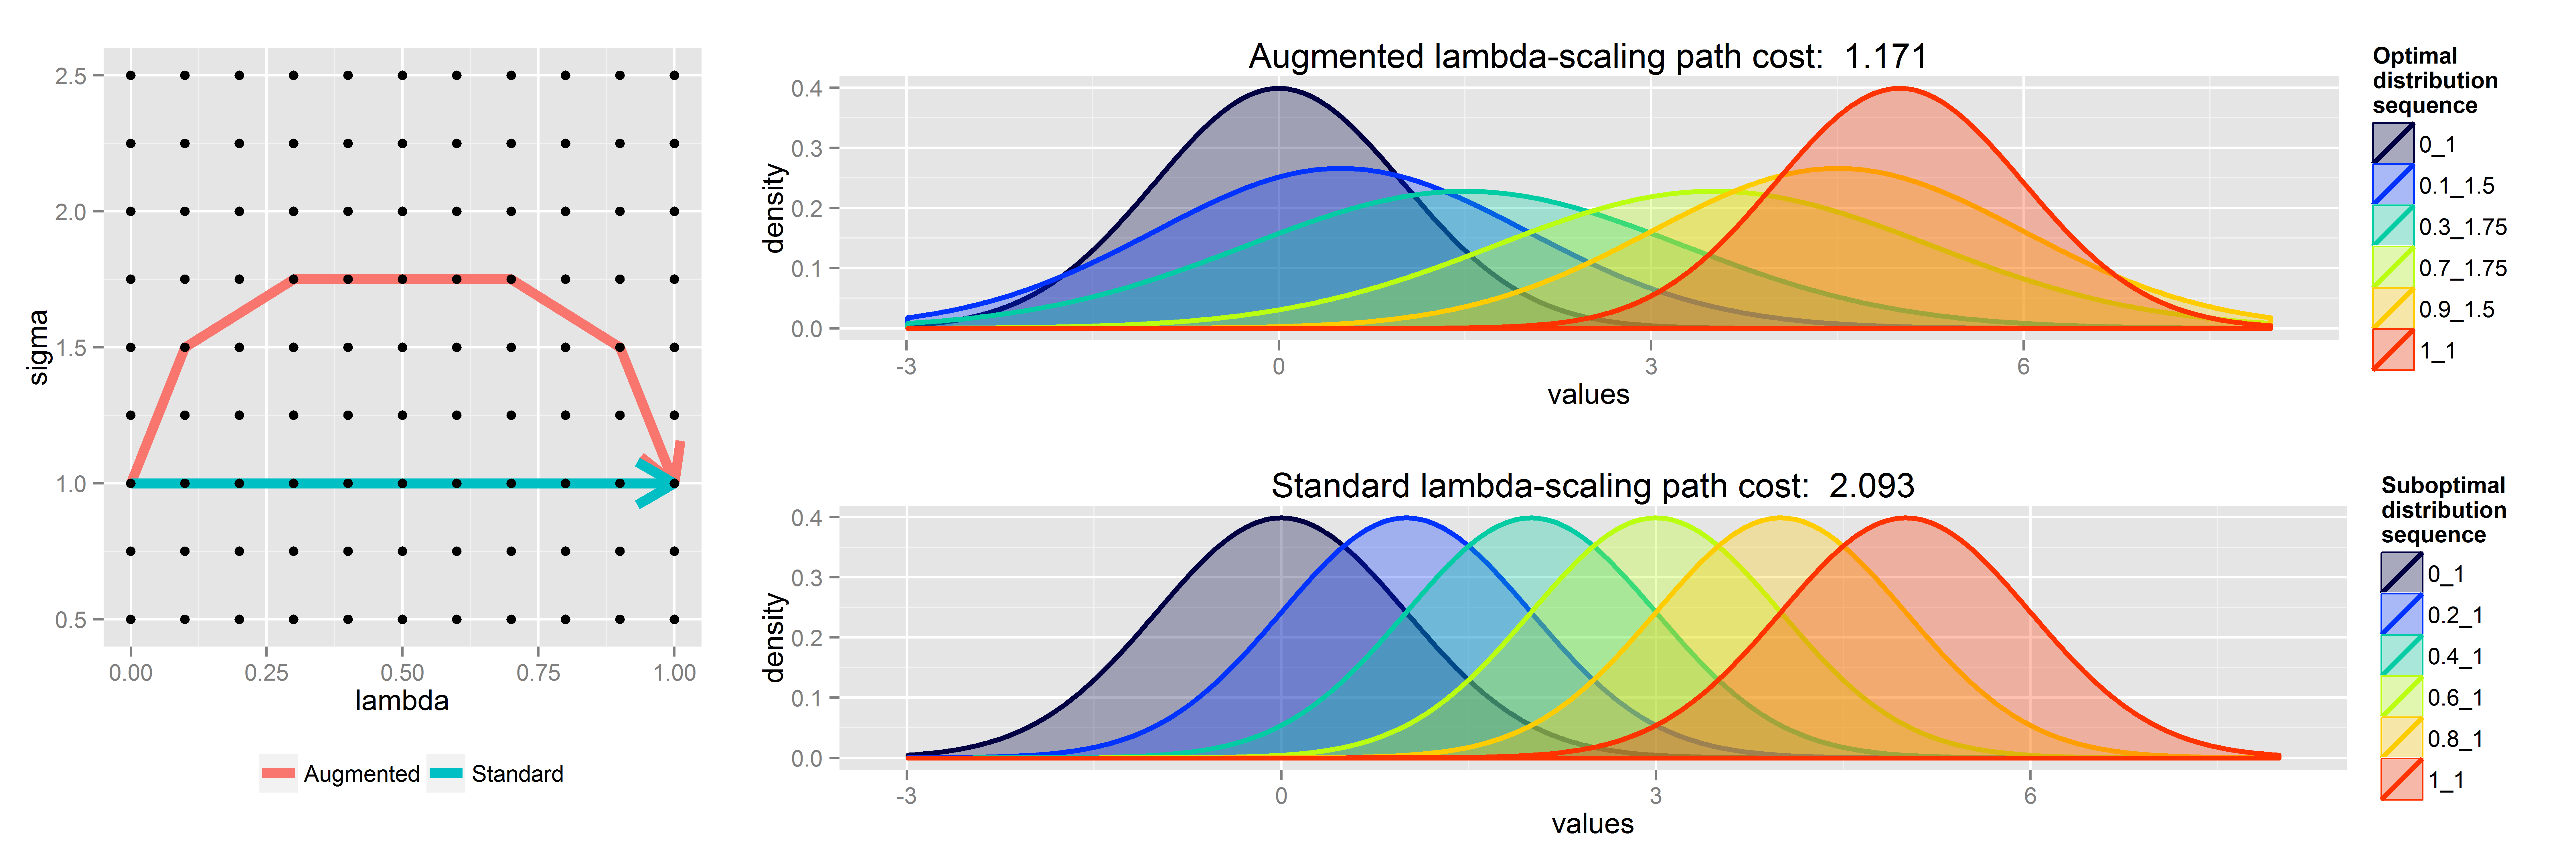
\includegraphics[scale=0.4]{unimod-3pan-searchv2.png}
\caption[Dijkstra search on total variation distance for offset harmonic wells]{Dijkstra search on total variation distance for offset harmonic wells. Left panel: Parameter representation of paths. Optimal path for temperature augmented $\lambda$-space in red. Optimal path for standard, one dimensional, $\lambda$ space in blue. Right panel: Density representation of paths. Top panel: distributions along optimal path flatten with increased temperature. Path cost of 1.171. Bottom: distributions along standard path simply mean shift. Path cost of 2.093.}
\label{uniuni}
\end{figure}

The result of the search are shown in figure \ref{uniuni}. We show that in discrete spaces, the Gelman and Meng result holds. An ellipsoid path which raises the temperature for intermediate distributions is the overall optimal path. These results confirm that not only is the standard path suboptimal, but that it is direly so. The path cost of the best standard solution is 2.093, which is nearly a two-fold increase from the globally optimal solution of 1.171.

To confirm the general utility of the augmented $\lambda$ space, we repeated the above search for a different target distribution, representing an increase in complexity. We set $U_1(x) ~\propto~ (ax^4-bx^2)$, where $a$ and $b$ are arbitrary scalars, to create a bimodal distribution. 
The result of this search, shown in figure \ref{unibi}, is consistent with that from figure \ref{uniuni}. The general shape of the optimal path appears to be somewhat conserved: high temperature regions are leveraged to increase distributional overlap.

\begin{figure}
\centering
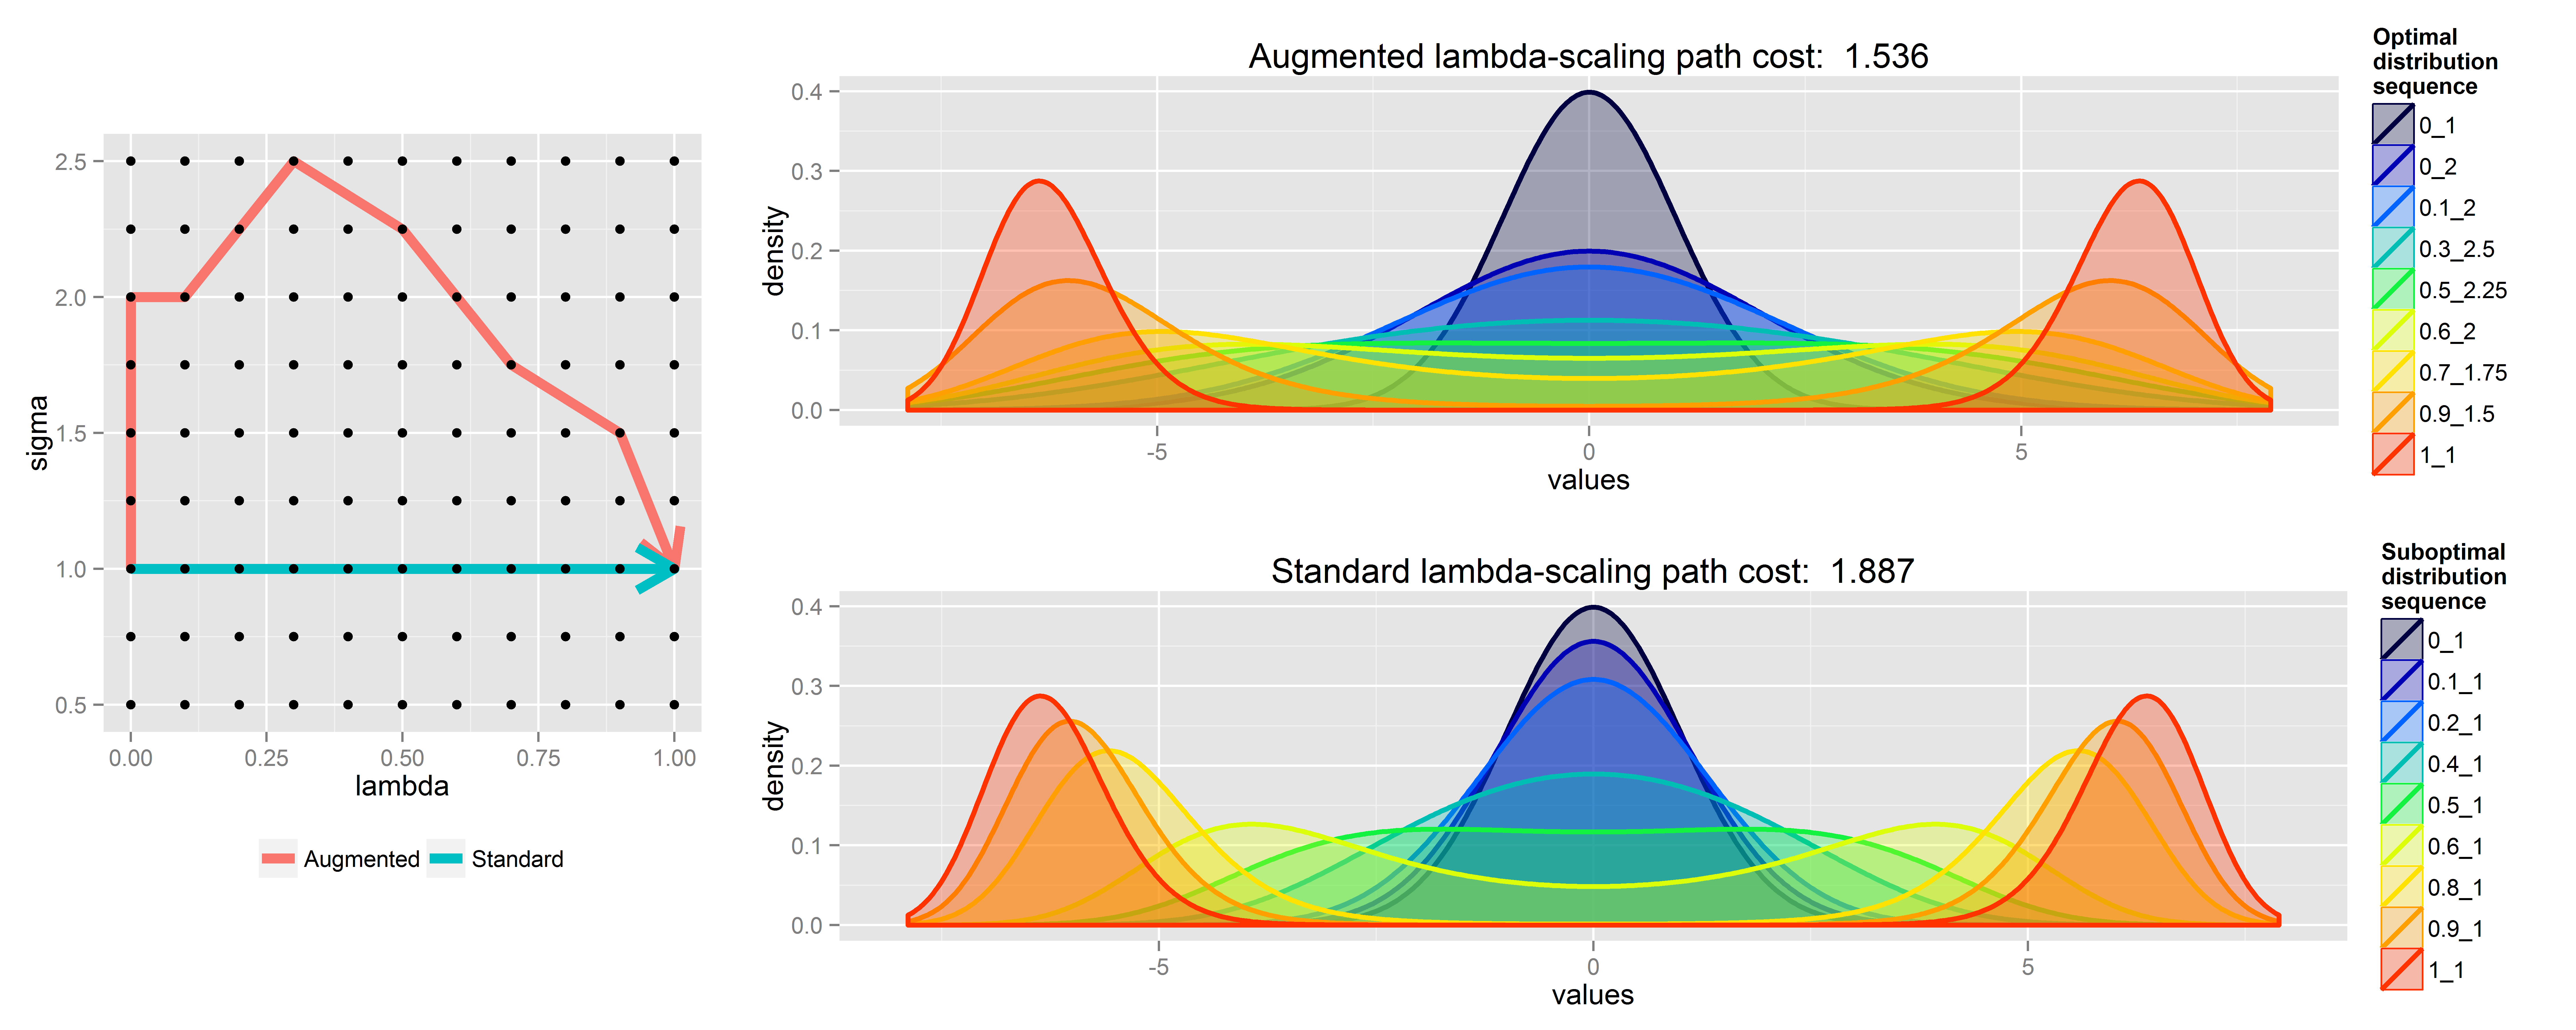
\includegraphics[scale=0.4]{unib1-3pan-searchv1.png}
\caption[Dijkstra search on total variance distance for the normal to bimodal transformation]{Dijkstra search on total variance distance for the normal to bimodal transformation. Panels mirror those from figure \ref{uniuni}. Optimal path cost: 1.536. Standard path cost: 1.887.}
\label{unibi}
\end{figure}

\section{Moving towards free energy calculations}

\subsection{A proper distance metric - varBAR}

In the previous section, we used total variation distance as edge weights in the graph search. 
While informative, this does not accurately reflect the type of information available for macromolecular systems. 
As the goal of a free energy calculation is to minimize the variance of the free energy estimate, a more appropriate distance metric is exactly that: the variance of the BAR estimate between adjacent states (hereafter the varBAR distance).
For the BAR estimator, an expression for the asymptotic variance of the free energy difference (or equivalently, the relative variance of the ratio estimate) was derived by Shirts and his colleagues\cite{shirts2008statistically, shirts2003equilibrium}:

\begin{equation} \label{eq:varbar}
    \text{var}(\Delta \hat{f}) = \frac{\text{var}(\hat{r})}{r^2} = \frac{1}{N}\left [ \left \langle \frac{1}{2+2\cosh(\Delta \hat{f} - \Delta u(x) -M)} \right \rangle ^{-1} - \left ( \frac{N}{N_2} + \frac{N}{N_1} \right ) \right ]
\end{equation}

\noindent where $M=\ln N_1/N_2$. Empirical tests show that this expression returns accurate variance estimates even for limited sample sizes.% (data not shown).

\begin{figure}
    \centering
    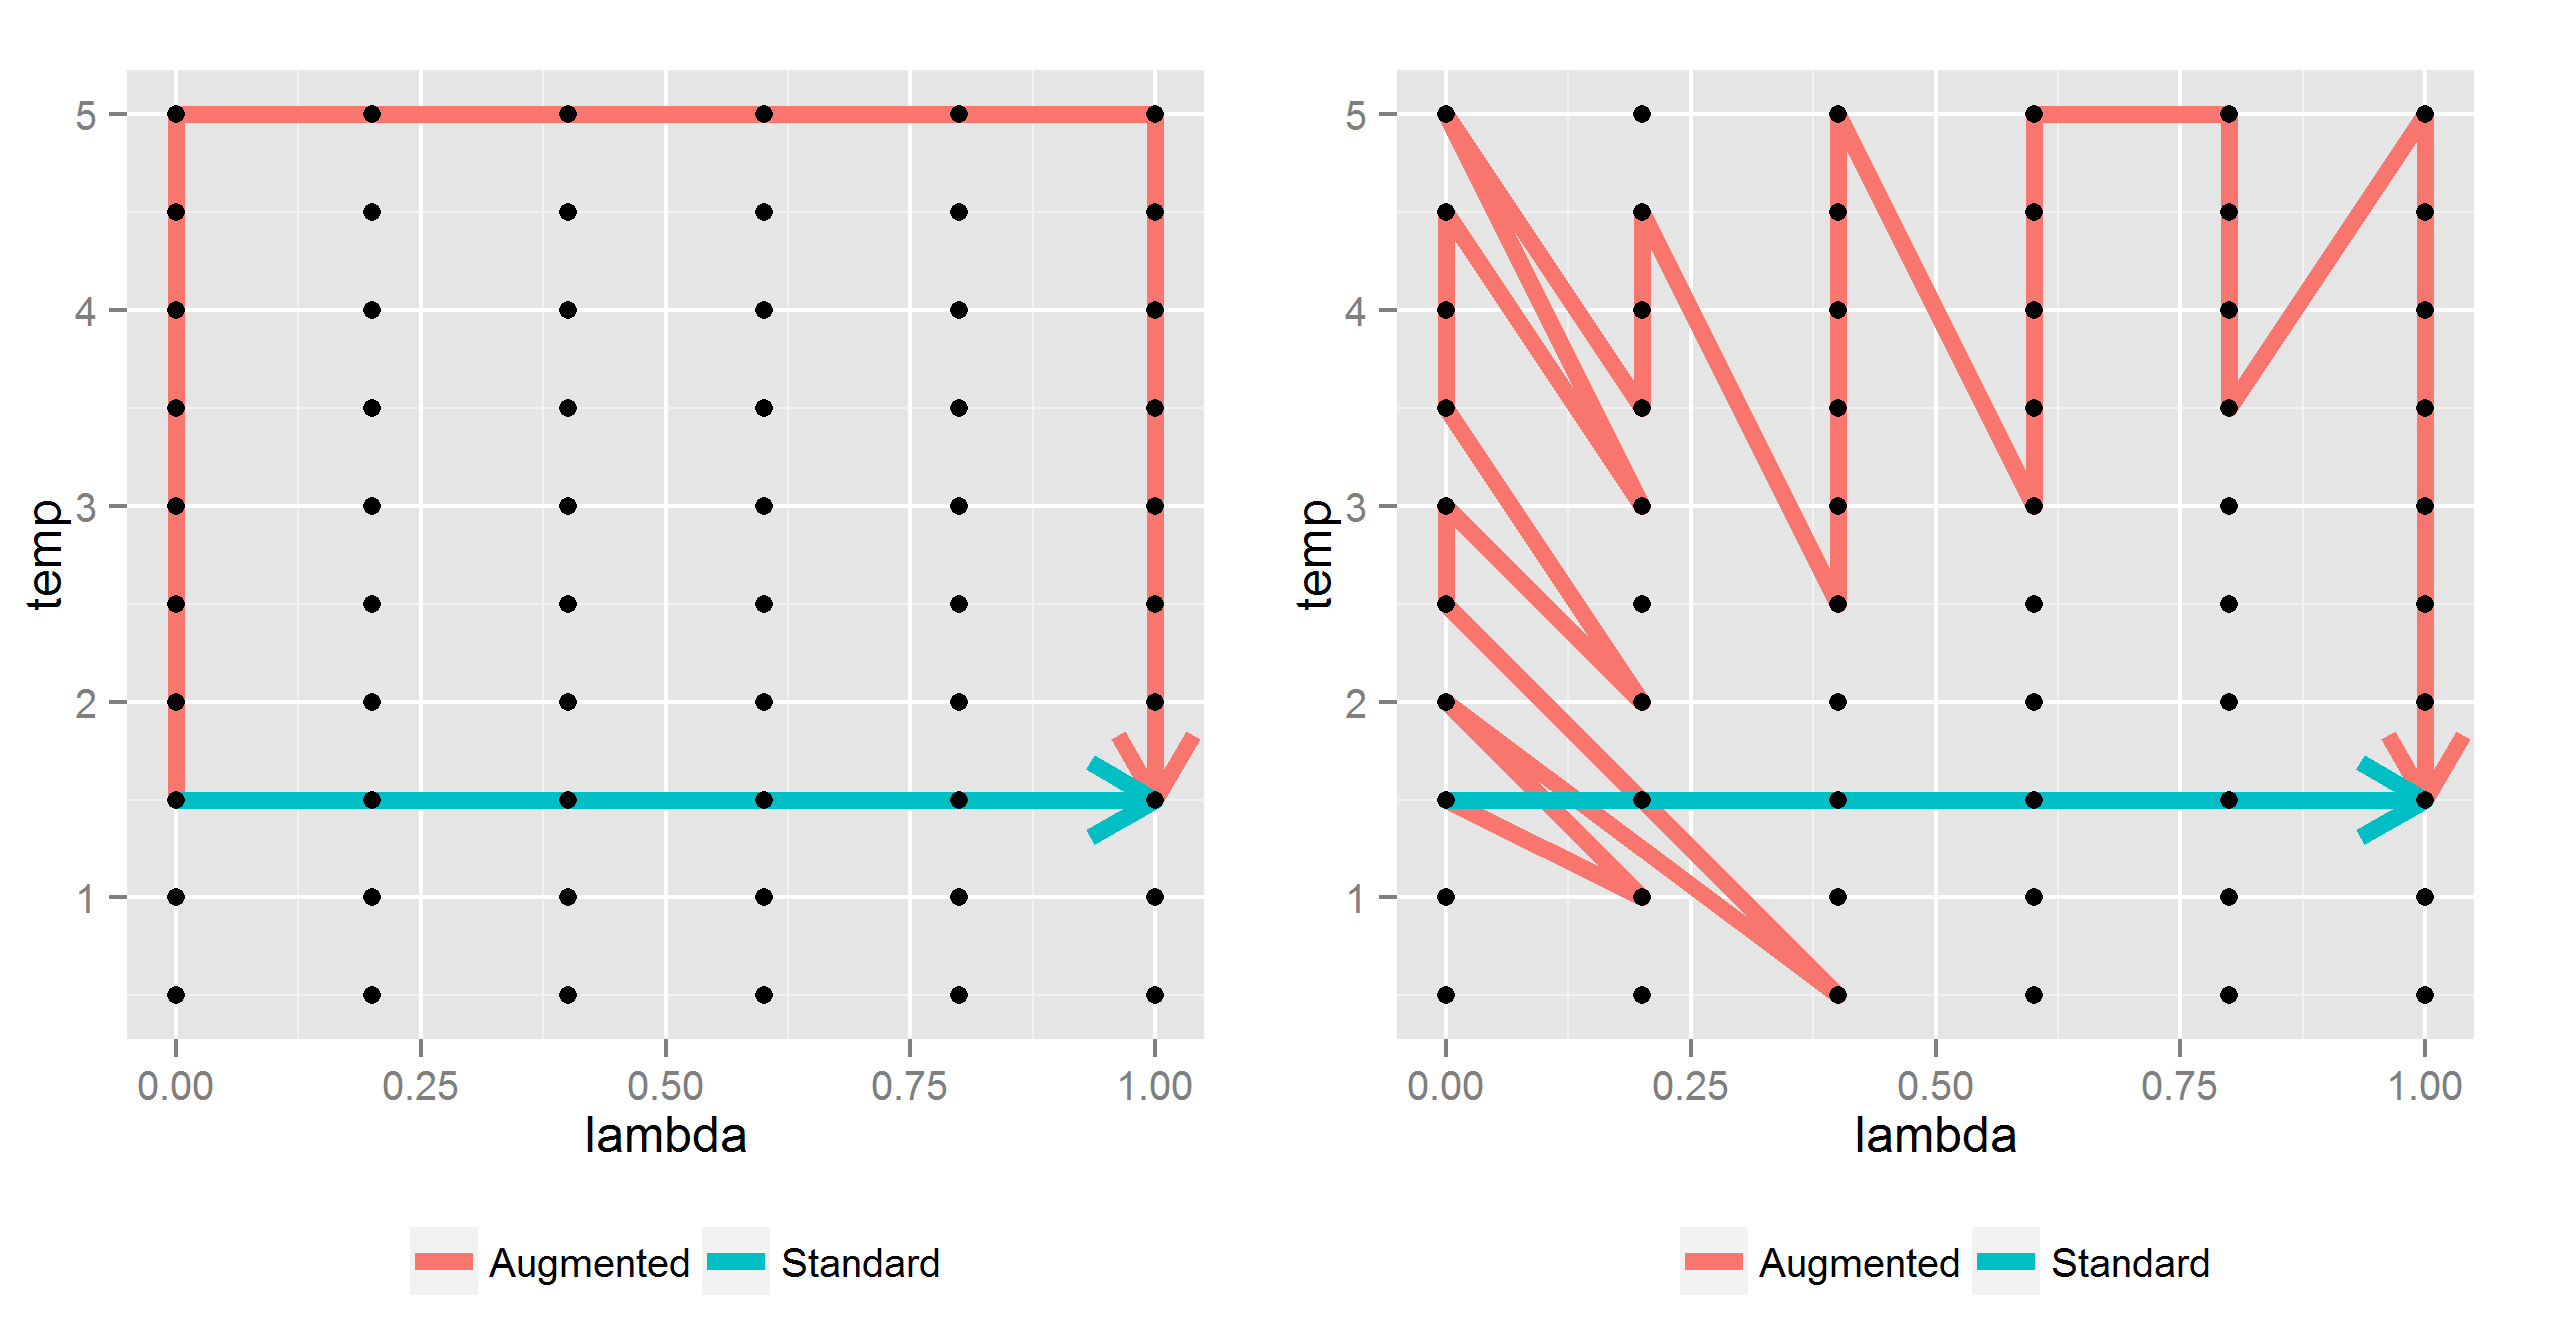
\includegraphics[scale=0.2]{varBAR-paramviews.png}
    \caption[Dijkstra search on varBAR distance]{Parameter representation of paths for Dijkstra search on varBAR distance for offset harmonic wells (left) and normal to bimodal transformation (right). See text for path costs.}
    \label{varbar-paramviews}
\end{figure}

Figure \ref{varbar-paramviews} summarizes the search results using this new objective function for the previously examined test cases. 
For the normal to normal case, the optimal path cost is 5.13E-4, and the standard path cost is 1.58E-3. For the normal to bimodal case, the optimal path cost is 3.93E-4, and the standard path cost is 1.81E-3.
While the variance is substantially reduced in both cases (approximately 70\% and 80\% reduction in variance respectively), we note that both optimal paths contain many intermediate states.
In a molecular simulation context, these paths would incur a much higher sampling cost, due to the number of intermediate states requiring simulation.
Indeed, if we add intermediates to the standard path to match the number of intermediates in the optimal paths, the benefit of the augmented space becomes unclear. 
The standard path costs for the normal to normal and normal to bimodal cases become 3.88E-4 and 2.18E-4, respectively.

\subsection{Cost adjusted paths}

In order to make sound comparisons, we must put a constraint on the total amount of computation, or equivalently, fix the total number of drawn samples across all paths being compared. 
In an equilibrium sampling context, depending on the total number of edges in a path, the number of available draws on each constituent state will vary, and consequently the cost of an edge will vary, due to variance scaling with N, as seen in \eqref{eq:varbar}. 
This dependence on global properties of the path on individual edge costs breaks the dynamic programming Dijktra's algorithm is built on.

To properly optimize these equal cost paths, we use a modified version of Dijkstra's algorithm, which constrains paths to a fixed length, then carry out a search for a range of possible path lengths. % http://stackoverflow.com/questions/1690347/shortest-path-with-a-fixed-number-of-edges
By prespecifying the number of edges in the solution path, we can determine the number of samples per state, and scale all edge costs appropriately for a recursive dynamic programming search.

\begin{figure}
    \centering
    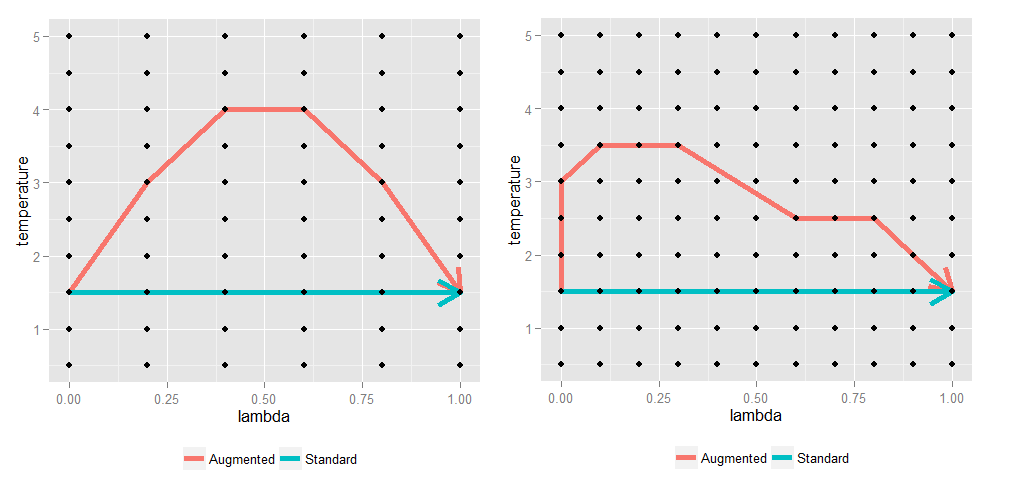
\includegraphics[scale=0.55]{kshortest.png}
    \caption[Cost-adjusted Dijkstra search]{Parameter representation of paths for cost-adjusted Dijkstra search on varBAR distance for offset harmonic wells (left) and normal to bimodal transformation (right). See text for path costs.}
    \label{fig:kshortest}
\end{figure}

Figure \ref{fig:kshortest} shows the optimal paths when varBAR costs account for the total number of edges in the path. 
For the offset harmonic well, the standard path cost is 5.07E-4, and the augmented path cost is 3.18E-4. 
For the unimodal to bimodal case, the standard path cost is 7.03E-5, and the augmented path cost is 5.93E-5.
We note that these corrected paths regain some of the smoothness that we had observed in figures \ref{uniuni} and \ref{unibi}.


\section{Scalability of Dijkstra's algorithm to molecular systems}

The results from this chapter serve as a proof of concept and establish the validity and theoretical utility of the temperature augmented state space for free energy calculations, however Dijkstra's algorithm is not suitable for path optimization going forward.
Dijkstra's algorithm requires knowledge of every edge weight in the graph.
Consequently, in order to apply Dijkstra's algorithm, a sufficient number of samples must be drawn from each alchemical state.
For molecular systems, this type of exhaustive search is cost prohibitive, and a path searching methodology which balances exploration and exploitation to discover and refine paths online is necessary. 
We will revisit our options for path selection in chapter \ref{chap:ql}.

